\chapter{Análisis del espectro EM en la banda de FM}
\section{Banda FM}
La banda de radio FM va desde 88 a 108 MHz -entre los canales de televisión
VHF 6 y 7-. Las estaciones de FM tienen asignadas frecuencias centrales
empezando en 88,1 MHz, con una separación de 200 KHz, y un máximo de 100
estaciones. Estas estaciones de FM tienen una desviación máxima de su frecuencia
central de 75 kHz, lo cual deja unas "bandas guardas" superior e inferior
de 25 kHz, para minimizar la interacción con las bandas de frecuencias adyacentes.

\begin{figure}[ht]
    \begin{center}
        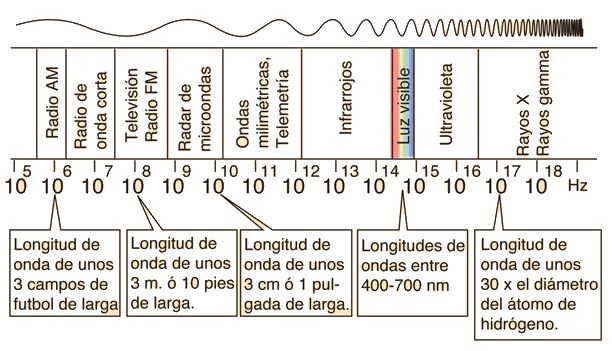
\includegraphics[scale= 0.7]{contenido/img/ej6espectrofm.jpg}
        \caption{El espectro electromagnético}
    \end{center}
\end{figure}

\begin{figure}[ht]
    \begin{center}
        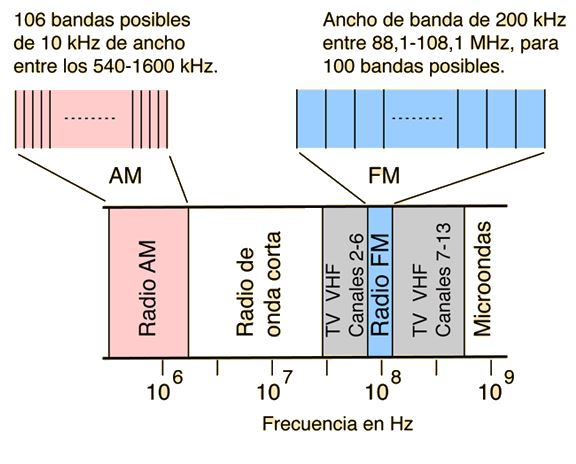
\includegraphics[scale= 0.7]{contenido/img/ej6espectroradio.jpg}
        \caption{El espectro de canales de radio}
    \end{center}
\end{figure}

\section{Banda de Radiodifusión de FM Estéreo}
El ancho de banda asignado a cada estación de radio FM, es
suficientemente amplio para la difusión de señales en estéreo de
alta fidelidad. La frecuencia de la portadora está modulada
directamente, con la suma de las señales de sonido de los canales
izquierdo y derecho. Una subportadora de 38 kHz, tambien modula la
portadora y esa subportadora, está modulada con la diferencia de
las señales de audio de los canales izquierdo y derecho. El
sintonizador de FM decodifica luego esta señal y la separa en
los canales de audio izquierdo y derecho.

\begin{figure}
    \begin{center}
        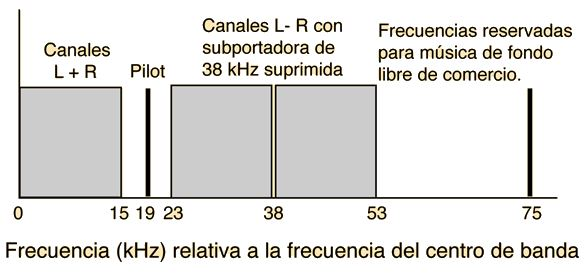
\includegraphics{contenido/img/ej6fig3.JPG}
    \end{center}
\end{figure}